
\section{Referring Expression Segmentation}
\vspace{-2mm}
The Referring Expression Segmentation task aims to segment a target object in an image or a video by understanding a given natural expression.

\subsection{Referring Image Segmentation}
% Early works, \cite{seo_urvos_2020} first extracted the visual and linguistic features and then directly fused and upsample two modalities to obtain the final segmentation predictions.

% Attention mechanism attracts more and more research fields due to its efficiency and effectiveness. VLT\cite{ding_vision-language_2021} employs an encoder-decoder attention network to enhance global context information. 

% Recently, CRIS\cite{wang_cris_2022} transfer multi-modal powerful knowledge of CLIP\cite{radford_learning_2021} for achieving text-to-pixel alignment.
\vspace{-2mm}
Referring Image Segmentation was first introduced by \cite{hu_segmentation_2016}, which aims to segment a target object or stuff in an image given a natural language expression. Early works proposed extracting the visual and linguistic features independently from CNN and RNN, respectively, and then concatenating them together to gather multi-modal features and generating the final segmentation results by a decoder. Utilizing the successful of instance segmentation, \cite{yu_mattnet_2018} proposed a two-stage method that first generates a set of candidate instances, then leverages the linguistic features as guidance for selecting the referred object from that set. 

Recent works\cite{ding_vision-language_2021, yang_lavt_2022} design a Transformer-based multi-modal encoder aiming to fuse the visual and linguistic features. It captures the interaction between vision and language information in the early phase. In \cite{ding_vision-language_2021}, the input image and language expression adaptively produce a set of queries, then these queries are used to generate the referred object mask through a Transformer decoder.

Different from previous methods, CRIS\cite{wang_cris_2022} leverages the knowledge of the CLIP\cite{radford_learning_2021} and text-to-pixel contrastive learning to improve the compatibility of multi-modal information and boost the ability of cross-modal matching. 
\subsection{Referring Video Object Segmentation}

% Referring video object segmentation

\begin{figure}
    \centering
    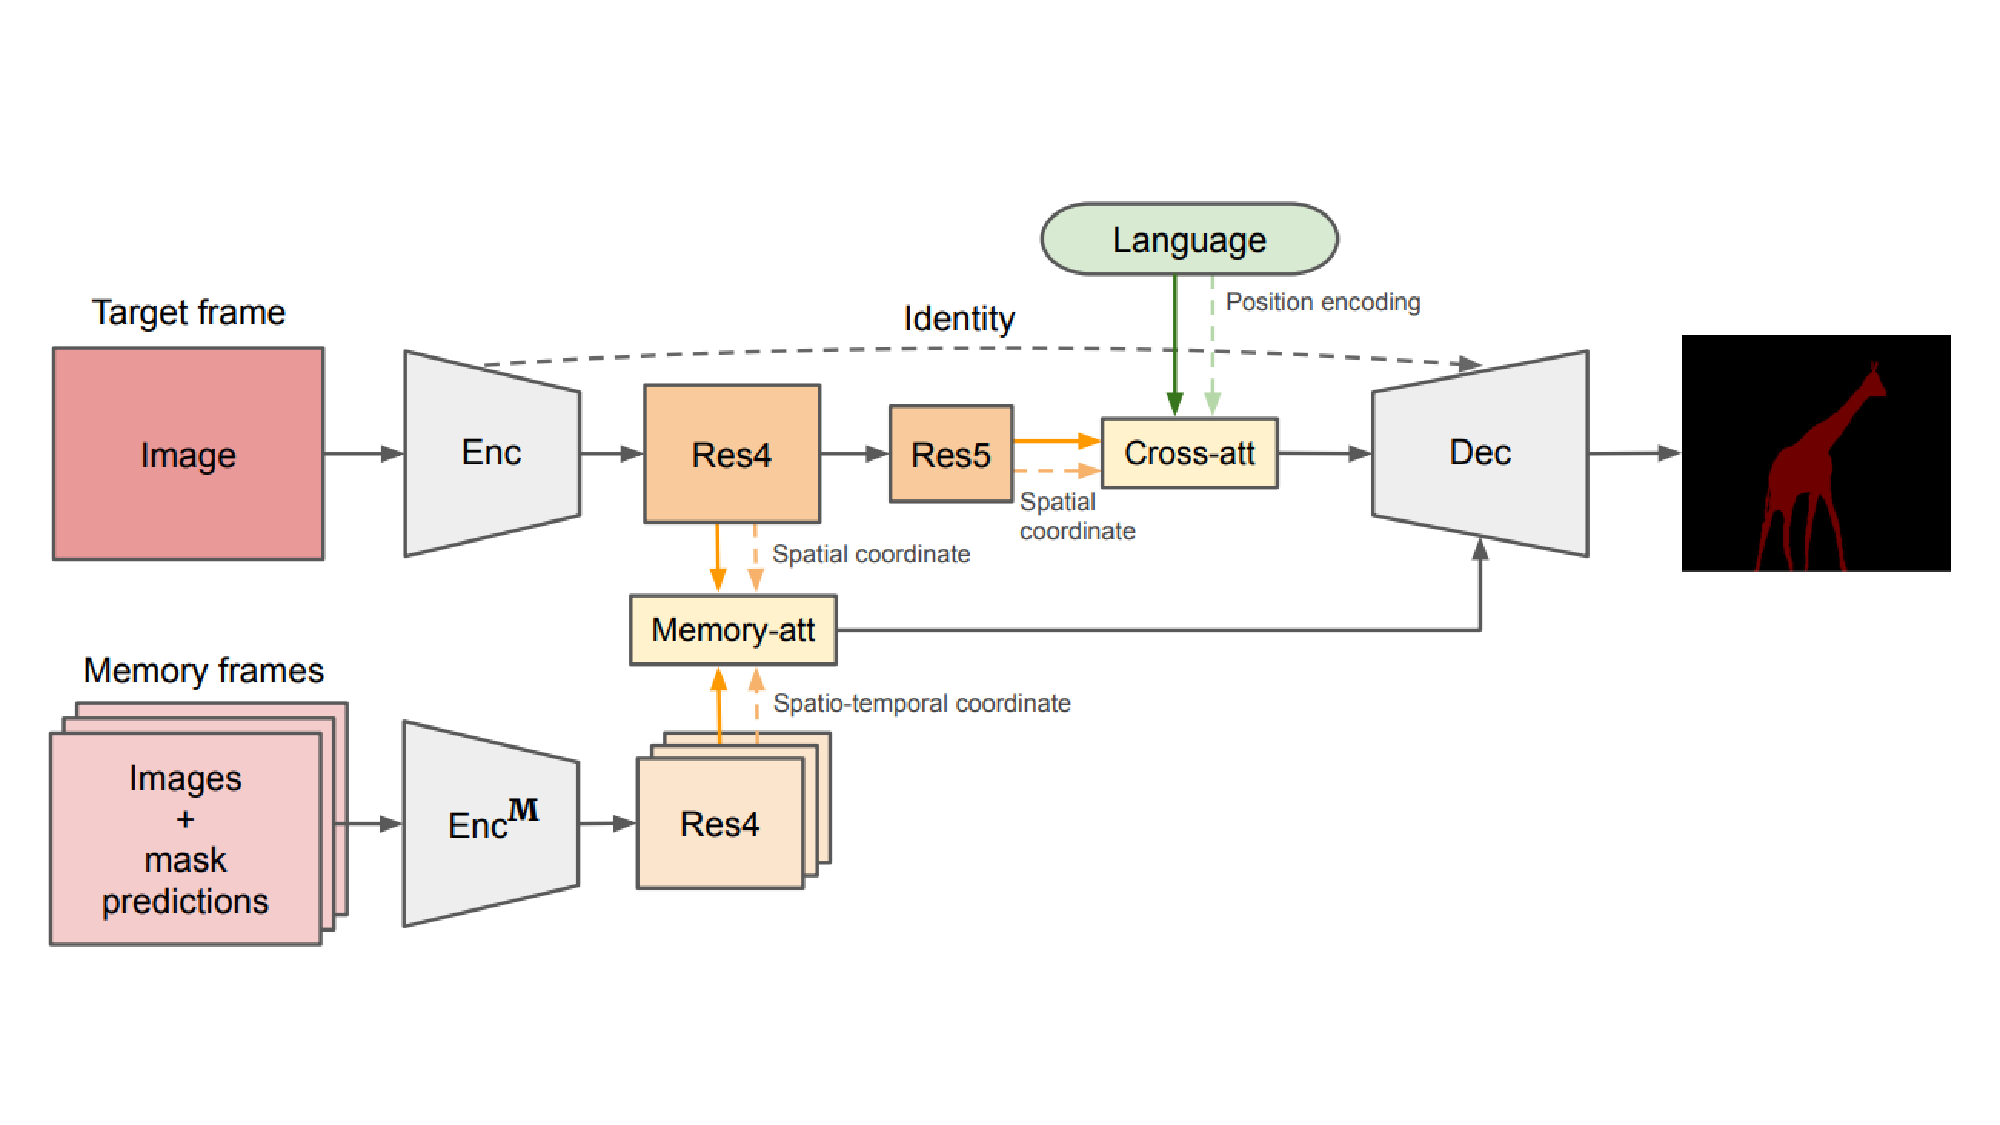
\includegraphics[width=0.8\textwidth]{content/resources/images/URVOS.pdf}
    \caption{Architecire overview of URVOS\cite{seo_urvos_2020}}
    \label{fig:urvos}
\end{figure}

The first common approach for referring video object segmentation is the bottom-up perspective. These methods apply the image-level referring methods \cite{seo_urvos_2020} directly on each video frame independently. The valuable temporal information across frames, therefore, can not be utilized. This obvious drawback leads to inconsistent object prediction due to the scene and appearance changes. URVOS \cite{seo_urvos_2020}(Figure \ref{fig:urvos}) leverages the mask propagation in a video besides the referring object segmentation in an image to address this issue. They propose a unified R-VOS framework that leverages the information of mask predictions in other frames by a memory attention module. 

The top-down method \cite{liang_rethinking_2021} first constructs a large set of object tracklets by propagating the object annotations detected and segmented from several keyframes to the whole video. Then, the best object tracklet is selected from the candidate set after associating with a language grounding model. Although the method achieves a breakthrough performance improvement compared to the previous methods, the complex and multi-stage pipeline makes it impractical and computational-expensive (Figure \ref{fig:top_down}).

\begin{figure}
    \centering
    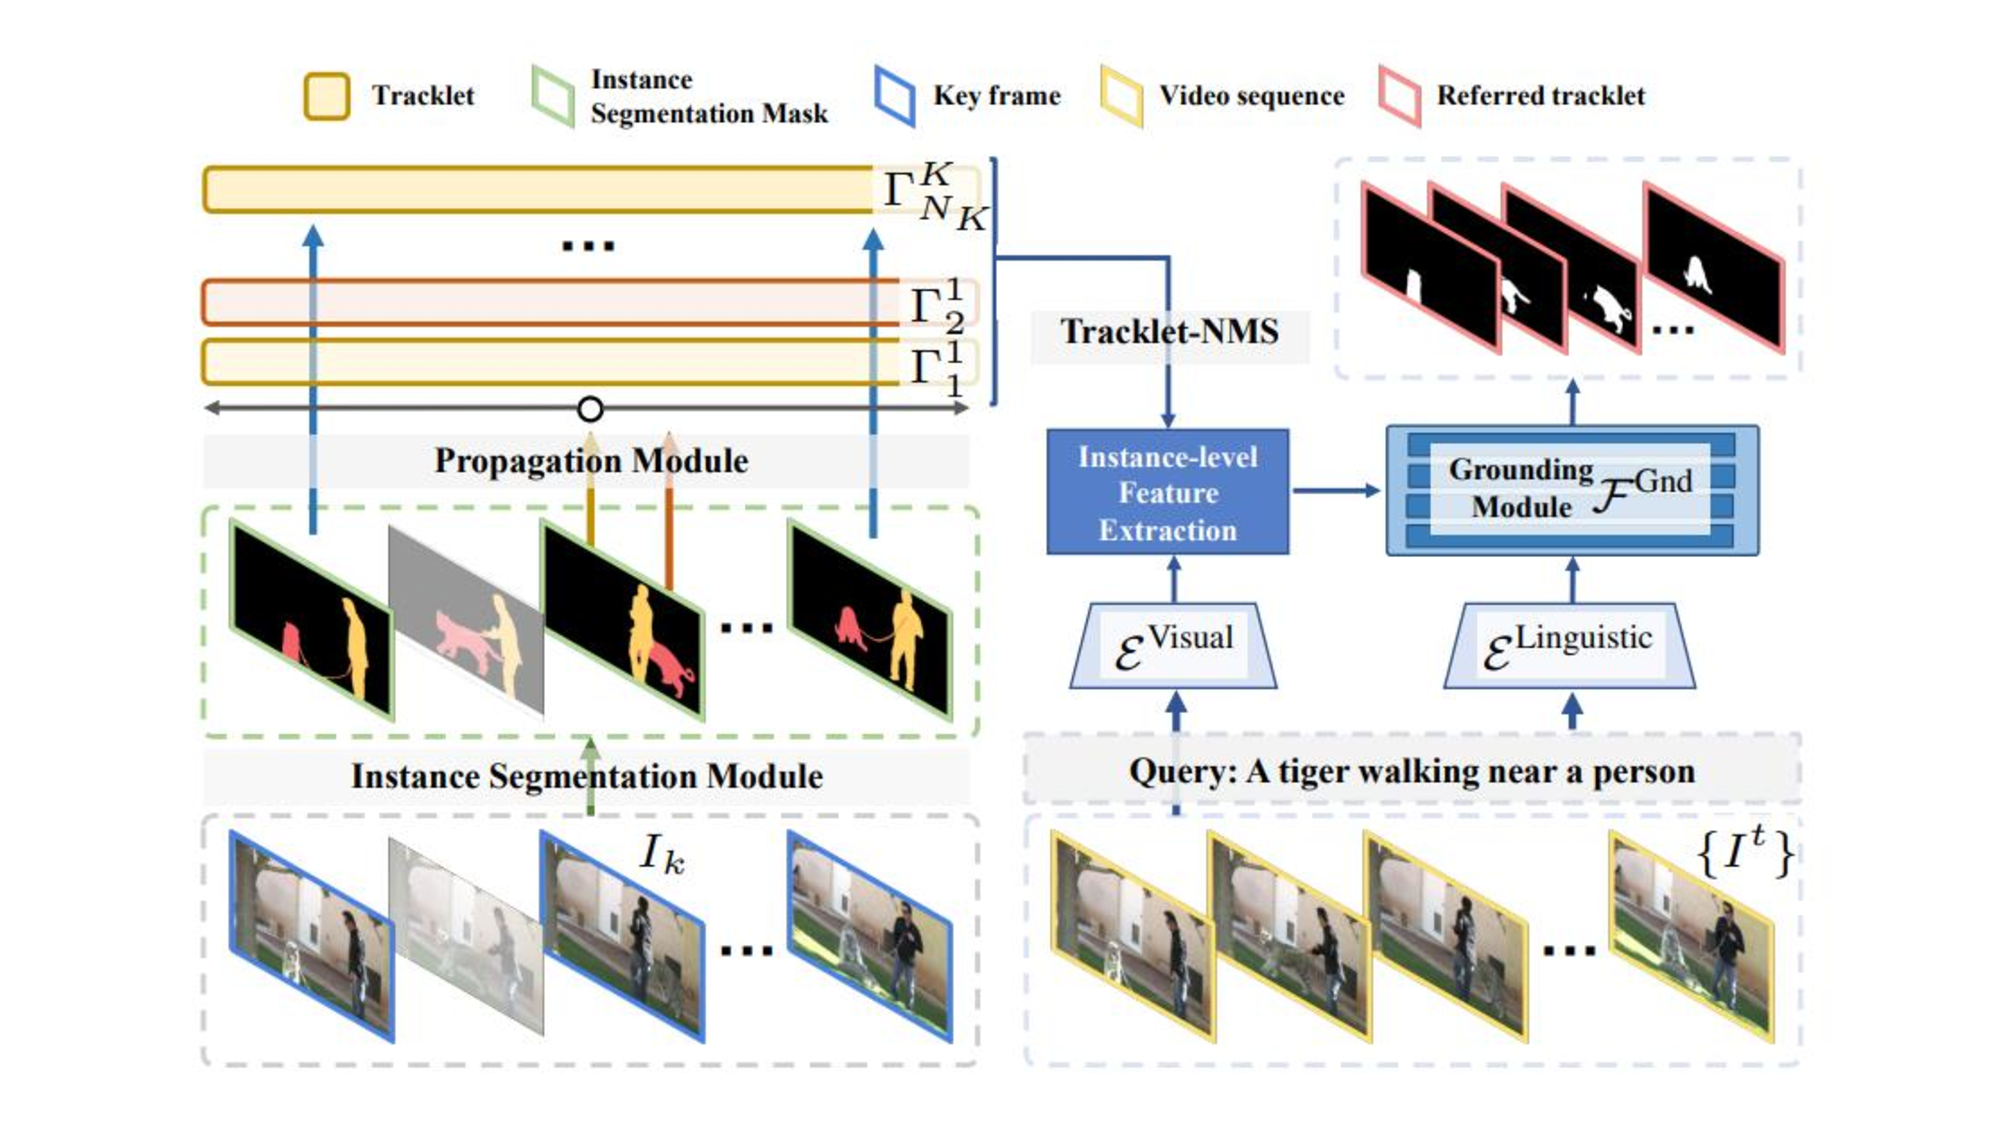
\includegraphics[width=0.8\textwidth]{content/resources/images/TopDown.pdf}
    \caption{Overall pipeline of Top-down method \cite{liang_rethinking_2021} }
    \label{fig:top_down}
\end{figure}

The query-based methods initialize a fixed set of object queries, then explore the global context of a video and relations between its frames and the language expressions via a Transformer decoder, and finally output a candidate set of predictions in parallel. MTTR\cite{botach_end--end_2022} first extract and concatenate the visual features from video frames and linguistics features from the language expression into multimodal sequences. A multimodal Transformer then encodes feature relations and decodes instances level features from a set of object queries into a set of prediction sequences. 


\begin{figure}[ht]
    \centering
    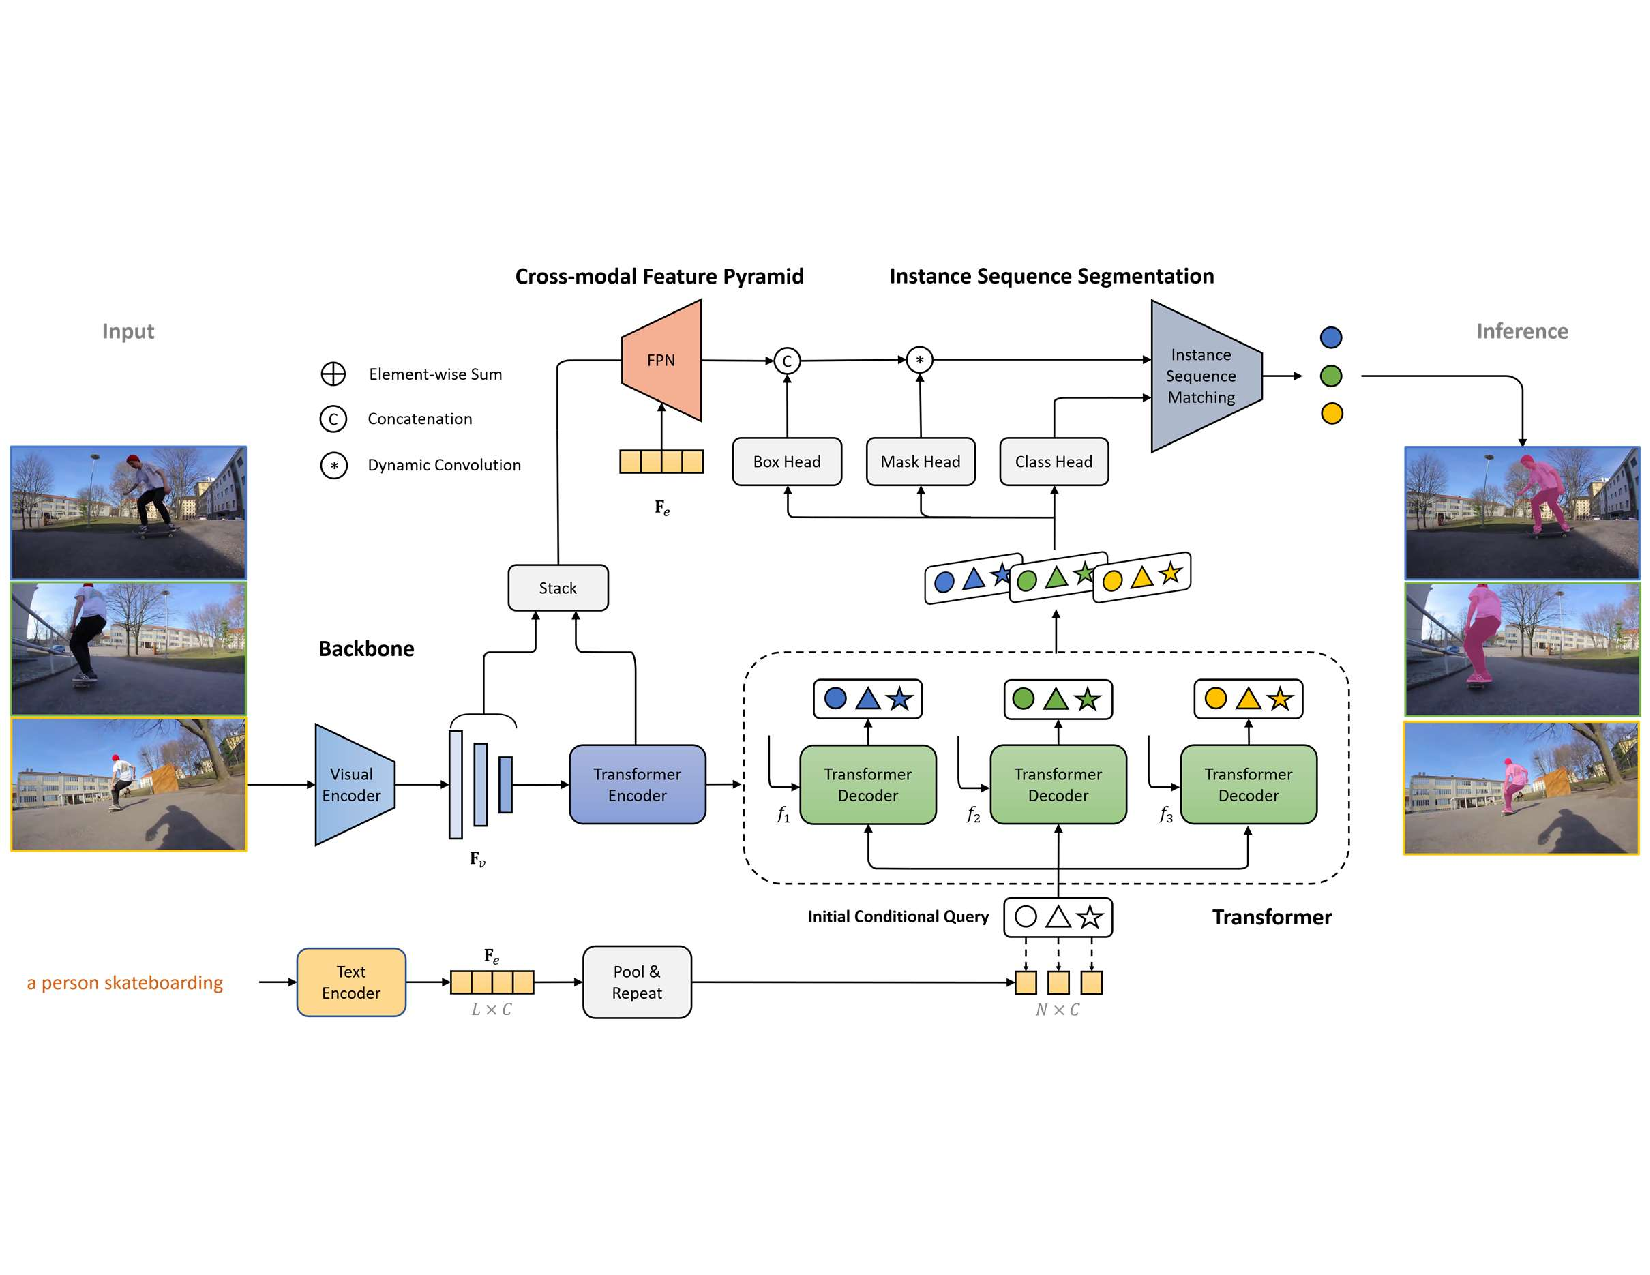
\includegraphics[width=\textwidth]{content/resources/images/ReferFormer.pdf}
    \caption{Overall pipeline of ReferFormer \cite{wu_language_2022} }
    \label{fig:referformer}
\end{figure}

\pagebreak
Another recently state-of-the-art model is the ReferFormer \cite{wu_language_2022}, which uses language as the initial queries to focus on the referred object only. Different from MTTR \cite{botach_end--end_2022}, ReferFormer uses the Deformable-DETR as its Transformer decoder due to its effectiveness and efficiency for global attention. Furthermore, Wu et al. \cite{wu_language_2022} utilized language information in the object queries, then they eliminated the linguistic features for the input of the Transformer decoder. Instead, Wu et al. proposed a Cross-modal Feature Pyramid Network for multi-scale vision-language fusion, improving mask features' quality for accurate segmentation (Figure \ref{fig:referformer}).  

Different from \cite{wu_language_2022, ding_vision-language_2021, yang_lavt_2022}, we do not leverage the visual and linguistic features for initializing the queries for Transformer decoder. Instead, we propose an Visual-Linguistic Transformer to aggregate the vision and language information into the object queries which effectively exploits the multi-modal features for enrich representation of object queries. 